
The position of the Sun in the sky, as observed from a given point on the Earth's surface, can be described
using two angles: the \textbf{solar altitude} \(\gamma_{\text{s}}\) and the \textbf{solar azimuth}
\(\alpha_{\text{s}}\). Let \(L\) denote the line connecting the observer's point on the Earth's surface to the
center of the solar disk and let \(\tilde{L}\) denote the projection of \(L\) onto the horizontal plane.
The solar altitude \(\gamma_{\text{s}}\) is the angle between \(L\) and \(\tilde{L}\) and the solar azimuth \(\alpha_{\text{s}}\)
is the angle between a line running in a true north-south direction and \(\tilde{L}\). In the Northern Hemisphere,
the solar azimuth angle is measured clockwise from due south, while in the Southern Hemisphere, it is measured
counterclockwise from due north. Values are negative before solar noon and positive after solar noon, corresponding
to positive values for directions west of the north-south line and negative values east of it \cite[p. 9]{CIBSE}.
This definition is used throughout the rest of the thesis, with the note that different conventions exist in
the literature. For example, Muneer \cite{Muneer} measures this angle positively clockwise from due north. Another important
angle is the solar zenith angle \(\psi_{\text{s}}\), which is the complement of the solar altitude angle relative to the
zenith direction, given by \(\psi_{\text{s}} = 90^\circ - \gamma_{\text{s}}\). The altitude angle is also referred to as the
elevation angle, indicating the elevation of the Sun above the horizon. Figure \ref{fig:SolarGeometry} illustrates
the solar geometry in relation to an oriented surface.

\begin{figure}
    \centering
    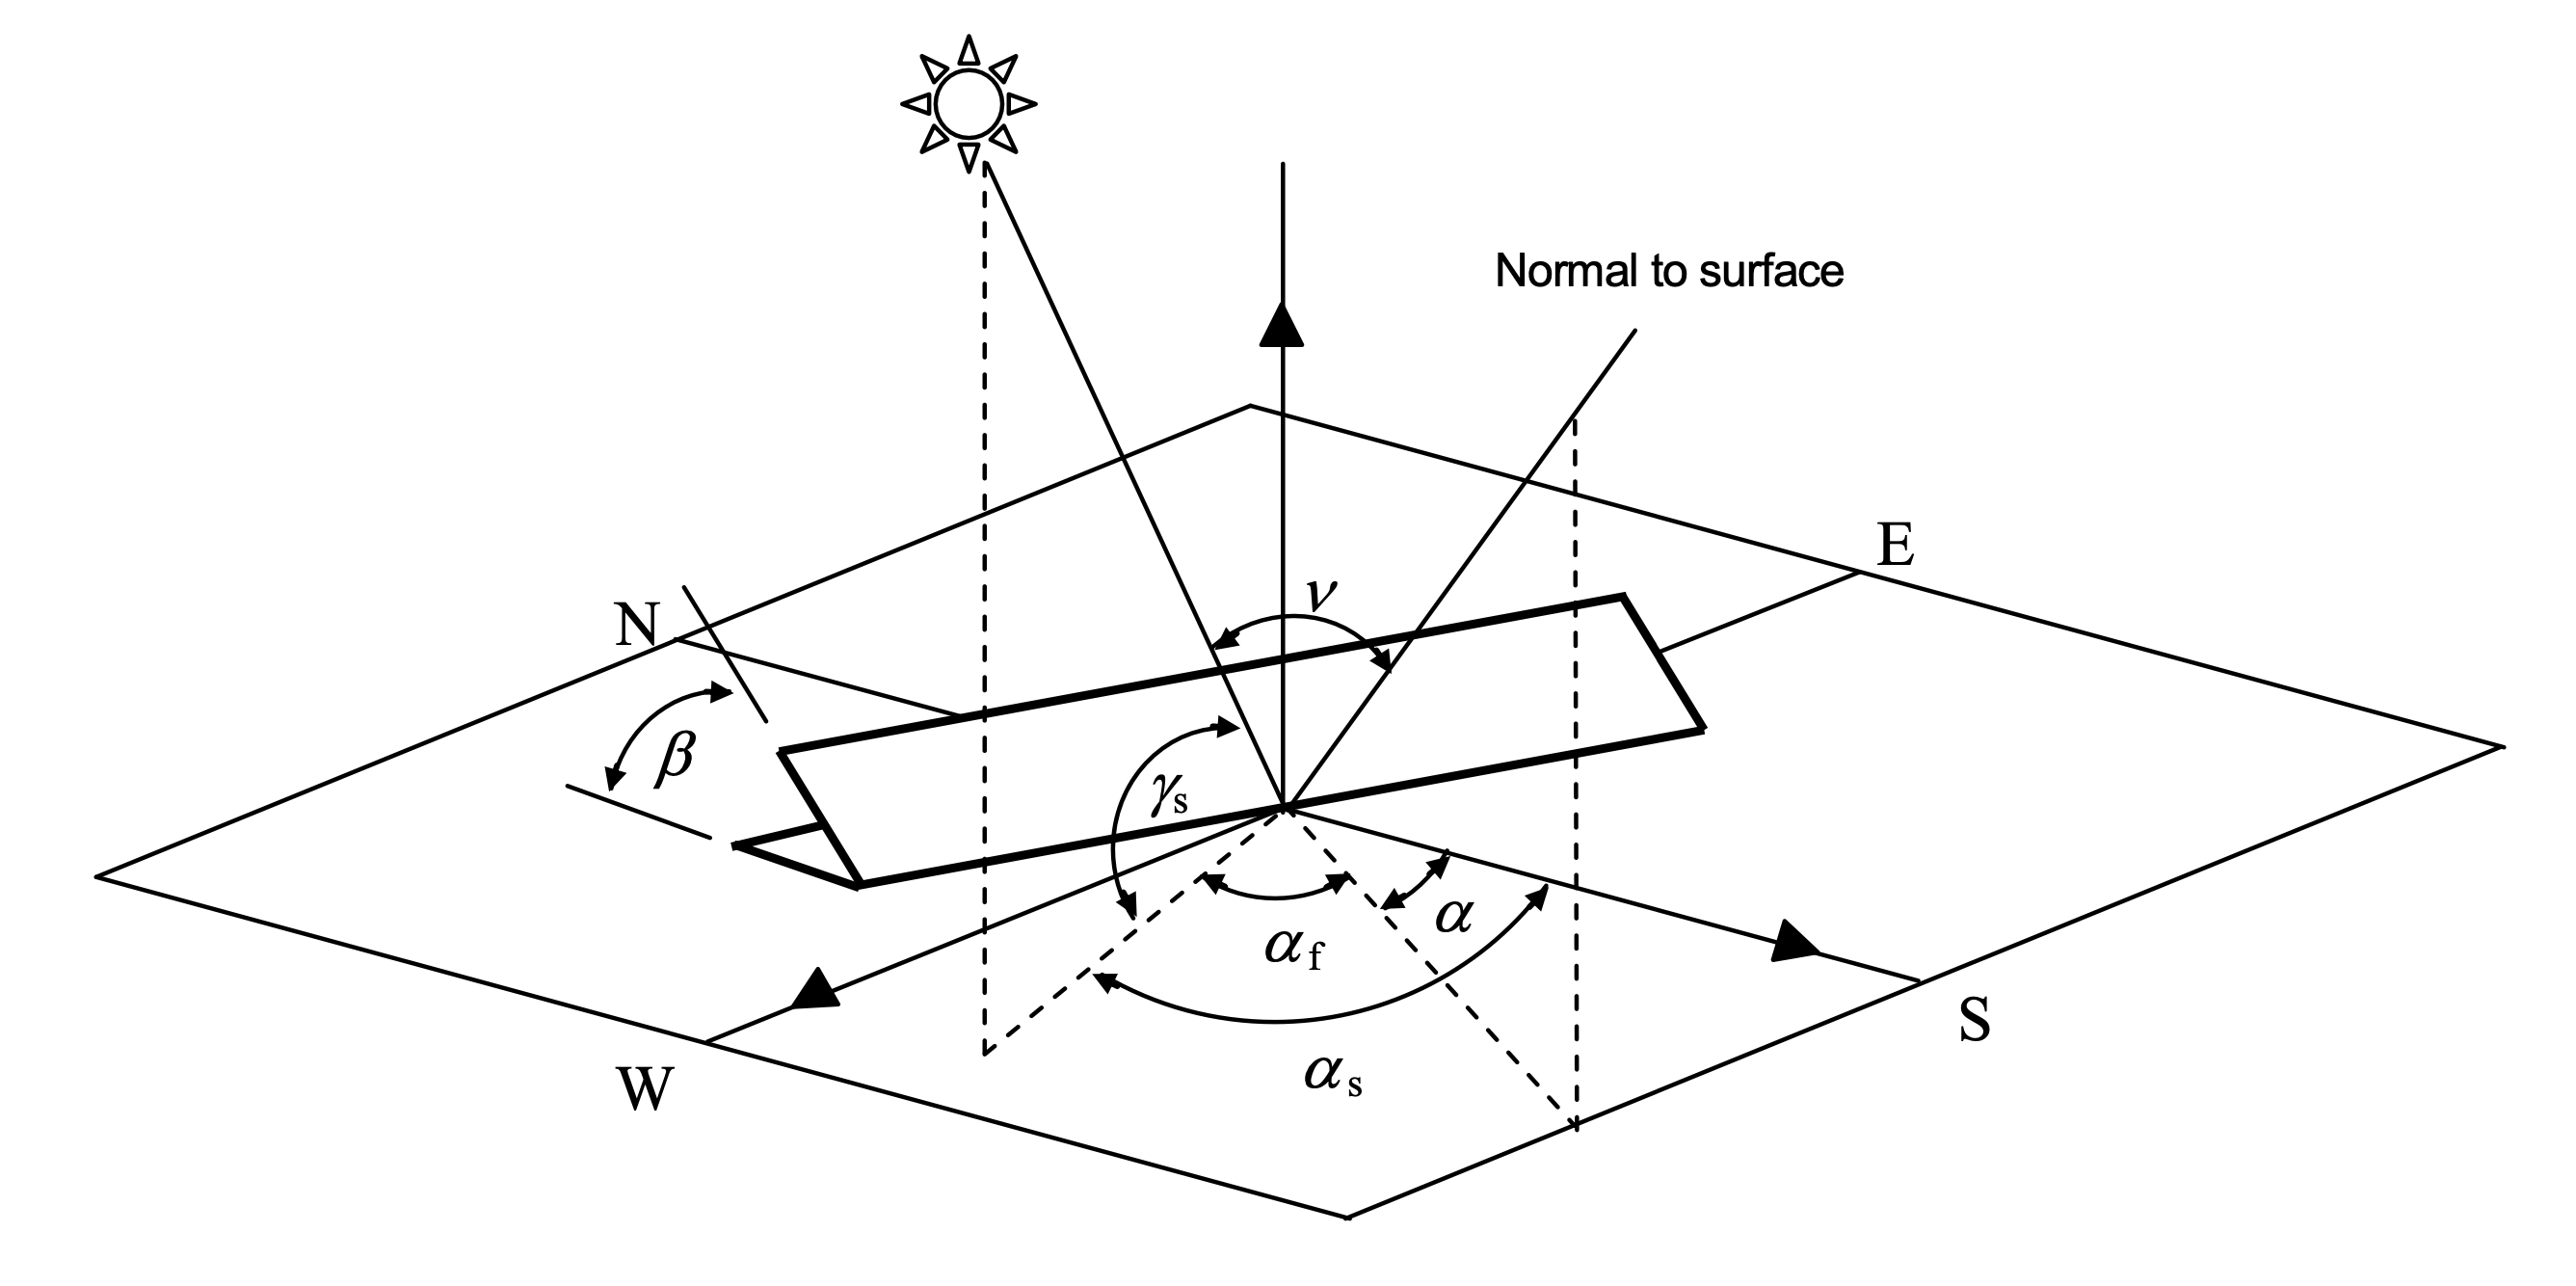
\includegraphics[scale=0.15]{Solar_Geometry_CIBSE}
    \caption{\small Solar geometry in relation to an oriented surface in the Northern Hemisphere \cite{CIBSE}.}
    \label{fig:SolarGeometry} % see https://www.overleaf.com/learn/latex/Inserting_Images
\end{figure}

As shown in the figure, the orientation of a surface can also be described using two angles: 
the surface tilt \(\beta\) and the surface azimuth \(\alpha\). The surface tilt angle \(\beta\) represents
the angular elevation of the surface from the horizontal plane, while the surface azimuth
angle \(\alpha\) describes the direction the inclined surface faces. Similar to the solar azimuth 
angle, different conventions exist in the literature. Throughout this work, the same  
convention as for the solar azimuth angle is used, as illustrated in the figure. For reference,
a selection of angle values and their interpretations is presented in Table \ref{tab:angles_and_values}.

\begin{table}
    \centering
    \begin{tabular}{rl@{\hspace{0.5cm}}rl@{\hspace{0.5cm}}rl}
        \toprule
        \multicolumn{2}{l}{\textbf{Surface tilt \(\beta\)}} & \multicolumn{2}{l}{\textbf{Solar altitude \(\gamma_{\text{s}}\)}} & \multicolumn{2}{l}{\textbf{Azimuths \(\alpha, \alpha_{\text{f}}, \alpha_{\text{s}}\)}} \\
        \midrule
        0°  & Surface horizontal & \hspace{0.05cm} 0°  & Sun behind the horizon  & \hspace{0cm}  0            & South          \\
        90° & Surface vertical   & \hspace{0.05cm} 90° & Sun directly overhead   & \hspace{0cm} -90°          & East           \\
            &                    & \hspace{0.05cm}     &                         & \hspace{0cm}  90°          & West           \\
            &                    & \hspace{0.05cm}     &                         & \hspace{0cm} ±180°         & North          \\
        \bottomrule
    \end{tabular}
    \caption{\small Selection of values of solar geometric angles and their interpretation for a 
        surface in the Northern Hemisphere. The roles of South and North are swapped
        in the Southern Hemisphere.}
    \label{tab:angles_and_values}
\end{table}

The positioning of the Sun relative to an oriented surface is described by the surface incidence angle 
\(\nu\), also known as the angle of incidence. This angle is defined as the angle between the normal
to the surface and the Sun's rays. It can be computed using the following three-step procedure 
\cite[p. 12]{CIBSE}:

\begin{enumerate}
    \item Calculate the wall-solar azimuth angle \(\alpha_{\text{f}} = \alpha_{\text{s}} - \alpha\)
    \item If \(\alpha_{\text{f}} > 180\) then \(\alpha_{\text{f}} = \alpha_{\text{f}} - 360\); if \(\alpha_{\text{f}} < 180\) then
    \(\alpha_{\text{f}} = \alpha_{\text{f}} + 360\)
    \item Calculate the incidence angle: \(\nu = \cos^{-1} \big(\cos\gamma_{\text{s}} \cos\alpha_{\text{f}} \sin\beta + \sin\gamma_{\text{s}} \cos\beta\big)\)
\end{enumerate}

Calculating the local Sun position angles \((\alpha_{\text{s}}, \gamma_{\text{s}})\), as introduced earlier, 
requires global Sun position coordinates that are independent of the observer's location: 
the Greenwich Hour Angle, the declination, and the right ascension \cite{Munner1993, Muneer1989}. 
These global coordinates describe the position of any celestial body in the sky. Their definitions 
are based on the concept of the celestial sphere, an abstract, imaginary sphere of arbitrarily 
large radius centered on the Earth. All celestial objects can be conceived as projected onto 
the surface of this sphere, simplifying the determination of their positions.
Orientation on the celestial sphere is defined by projecting Earth's poles and equator
onto the sphere, referred to as the celestial poles and celestial equator, respectively.
Declination and right ascension are analogous to latitude and longitude, representing angular
distances north or south and east or west, respectively. Right ascension is measured eastward
from the vernal equinox, the point where the Sun crosses the celestial equator at the March
equinox. Figure \ref{fig:Sun_global_coordinates_on_celestial_sphere} illustrates the concept
of the celestial sphere in relation to an arbitrary star.
As shown in the figure, the declination and right ascension of the Sun correspond to its
position as a point on the sphere along the projected Earth-Sun orbit. The final global
position angle, the Greenwich Hour Angle, represents the position of the Sun in the sky
relative to Earth's rotation. It is the angle measured westward from the Greenwich meridian
to the Sun's position. In this context, the Sun's position corresponds to the longitude
of the point directly beneath the Sun. This angle describes how far the Sun has moved
westward from the meridian.

\begin{figure}
    \centering
    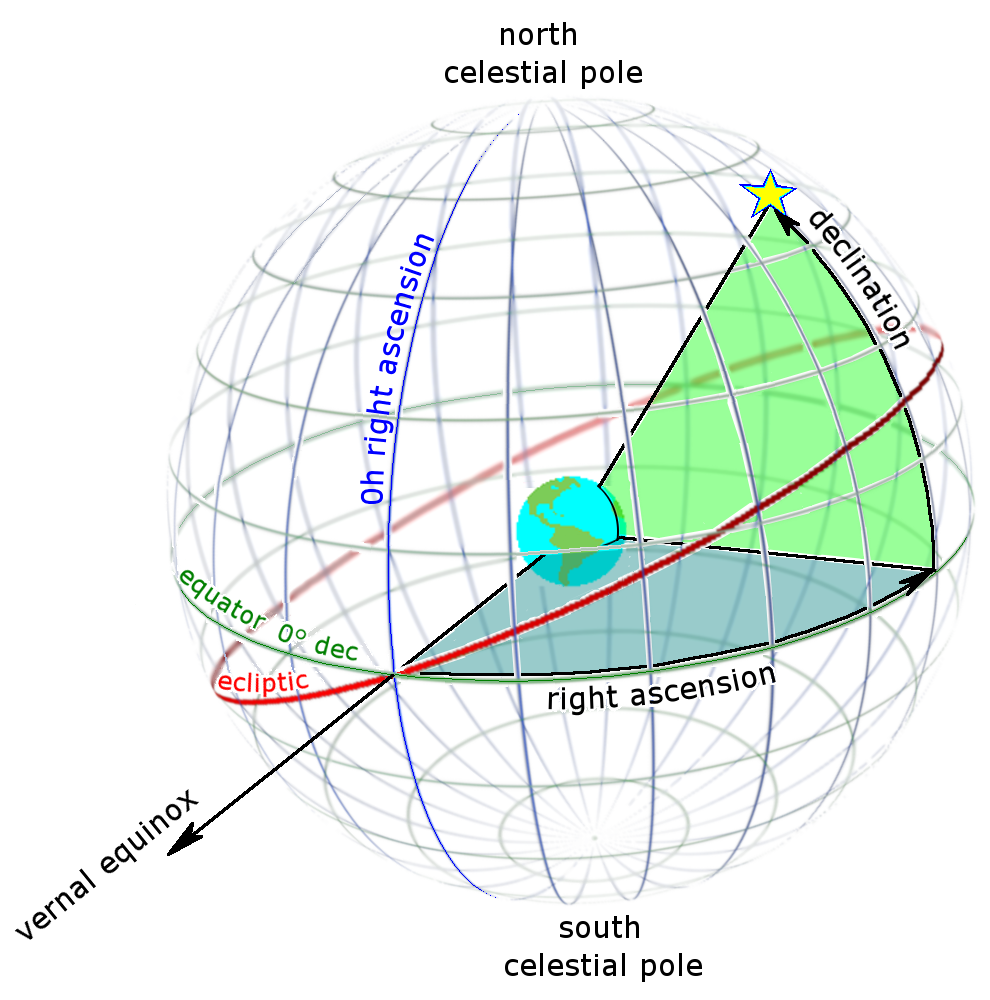
\includegraphics[scale=0.23]{Sun_global_coordinates_on_celestial_sphere.png}
    \caption{\small Visualization of global right ascension and declination \cite{WikipediaRightAscension}.}
    \label{fig:Sun_global_coordinates_on_celestial_sphere}
\end{figure}

Several factors affect the computation of the Sun's position, including the Earth's
axial tilt, which varies from 22 to 25 degrees over a period of approximately 41,000
years, and its orbital movement around the Sun, which alternates between a circular
and an elliptical orbit over a period of about 100,000 years. Additionally, the Earth
experiences a wobble, known as precession, in a cycle lasting around 23,000 years.
Gravitational interactions with the Moon and other planets, especially Jupiter and
Saturn, are primary contributors to these variations \cite[p.~2]{Muneer}. These and
other perturbations make accurate calculation of the Sun's position quite a difficult task.
The literature offers a wide variety of algorithms with different levels of accuracy
and complexity. Grena \cite{Grena} presents a set of five algorithms, valid from
2010 to 2100, that cover all possible applications in solar engineering. These
algorithms provide the Sun position angles \((\alpha_{\text{s}}, \psi_{\text{s}})\) in radians,
adhering to the conventions adopted in Section \ref{sec:Solar Geometry}. The
paper includes step-by-step descriptions optimized to reduce computational
complexity as much as possible. The calculations performed later
are based on the most accurate of these five algorithms, as the Sun's position
is required at sub-hourly intervals.

% \begin{table}[h]
%     \centering
%     \begin{tabular}{lcccc}
%         \toprule
%        \textbf{Panel type} & \textbf{Voc (V)} & \textbf{Isc (A)} & \textbf{Vmp (V)} \\
%         \midrule
%         Gruposolar GS601456P-218 & 36.30 & 8.19 & 29.00 & 7.55 \\
%         Kyocera KC175GHT-2 & 29.35 & 8.07 & 23.60 & 7.57 \\
%         Sanyo HIP-230 HDE1 & 42.46 & 7.26 & 34.00 & 6.87  \\
%         Shell S75 & 21.55 & 4.70 & 17.50 & 4.32 \\
%         \bottomrule
%     \end{tabular}
%     \caption{Data for the evaluation of the new model parameters.}
%     \label{table:model_parameters}
% \end{table}

% \begin{table}[h]
%     \centering
%     \begin{tabular}{lccccc}
%         \toprule
%         \textbf{Panel type} & \multicolumn{2}{c}{\textbf{Voc (V)}} & \textbf{Isc (A)} & \textbf{Vmp (V)} & \textbf{Imp (A)} \\
%         \cmidrule(r){2-3} % Draws a line under the Voc columns
%         & \textbf{Voc1} & \textbf{Voc2} & & & \\ % Voc1 and Voc2 are the new sub-column headers
%         \midrule
%         Gruposolar GS601456P-218 & 36.30 & (some value) & 8.19 & 29.00 & 7.55 \\
%         Kyocera KC175GHT-2 & 29.35 & (some value) & 8.07 & 23.60 & 7.57 \\
%         Sanyo HIP-230 HDE1 & 42.46 & (some value) & 7.26 & 34.00 & 6.87  \\
%         Shell S75 & 21.55 & (some value) & 4.70 & 17.50 & 4.32 \\
%         \bottomrule
%     \end{tabular}
%     \caption{Data for the evaluation of the new model parameters.}
%     \label{table:model_parameters_2}
% \end{table}

% \begin{table}[h]
%     \centering
%     \begin{tabular}{lccccc}
%         \toprule
%         \textbf{Panel type} & \multicolumn{2}{c}{\textbf{Voc (V)}} & \textbf{Isc (A)} & \textbf{Vmp (V)} & \textbf{Imp (A)} \\
%         \midrule
%         Gruposolar GS601456P-218 & 36.30 & (some value) & 8.19 & 29.00 & 7.55 \\
%         Kyocera KC175GHT-2 & 29.35 & (some value) & 8.07 & 23.60 & 7.57 \\
%         Sanyo HIP-230 HDE1 & 42.46 & (some value) & 7.26 & 34.00 & 6.87  \\
%         Shell S75 & 21.55 & (some value) & 4.70 & 17.50 & 4.32 \\
%         \bottomrule
%     \end{tabular}
%     \caption{Data for the evaluation of the new model parameters.}
%     \label{table:model_parameters_3}
% \end{table}

% \begin{table}[h]
%     \centering
%     \begin{tabular}{lccccc}
%         \toprule
%         \textbf{Panel type} & \multicolumn{2}{c}{\textbf{Voc (V)}} & \textbf{Isc (A)} & \textbf{Vmp (V)} & \textbf{Imp (A)} \\
%         \midrule
%         Gruposolar GS601456P-218 & 36.30 & (some value) & 8.19 & 29.00 & 7.55 \\
%         Kyocera KC175GHT-2 & 29.35 & (some value) & 8.07 & 23.60 & 7.57 \\
%         Sanyo HIP-230 HDE1 & 42.46 & (some value) & 7.26 & 34.00 & 6.87  \\
%         Shell S75 & 21.55 & (some value) & 4.70 & 17.50 & 4.32 \\
%         \bottomrule
%     \end{tabular}
%     \caption{Data for the evaluation of the new model parameters.}
%     \label{table:model_parameters_4}
% \end{table}

% \begin{itemize}
%     \item Global coordinates: solar declination and right ascension
%     \item Local coordinates: hour angle, solar altitude and azimuth 
% \end{itemize}

% The Greenwhich Hour Angle (GHA) is the angle measured westward of the
% Sun's position and the Greenwich meridian. In this context corresponds
% the Sun position to the longitude on which the point lies that is directly
% underneath the sun. This angle describes how far the sun moved westwards
% from the prime meridian. 

% Analogously to the GHA, the Local Hour Angle (LHA) measures how far the
% sun has moves westwards from the observers meridian. Hence it can be derived
% from the GHA and the observers longitude. 

% Solar time is a measure of time that depends on the position of the Sun in
% the sky. Solar noon occurs when the Sun is at its highest point in the sky,
% i.e. when the Sun crosses the local meridian. If it is 11 am solar time at
% a specific point on Earth, this means that the Sun is one hour away from solar
% noon for that location. Since the Earth rotates 15° of longitude per hour, the Sun is
% 15° to the east of the local meridian.

% The Equation of time (EOT) measured the time difference between solar time and
% the clock time.

% The solar day is the time between two successive solar noons and its length
% varies due to two main factors: the elliptical orbit of the earth and its
% axial tilt. As described by Kepler's law of planetary motion, the Earth's
% orbit around the Sun is not a perfect circle but an ellipse. This causes
% the Earth's speed in its orbit to vary: the Earth moves faster when it is
% closer to the Sun and slower when it is further away. This variation in
% speed causes the sun to appear more clickly (slowly) across the sky causing
% solar noon to arrive slightly earlier (later) each day.

% The declination angle is the angle between the equatorial plane and the line connecting
% the centres of the Sun and the Earth. It varies throughout the year due to the tilt
% of the Earth's axis relative to its orbit around the sun. The declination is positive
% in the Northern Hemisphere summer and negative in winter.

% The last global position angle, the Greenwhich Hour Angle, captures the position
% of the Sun in the sky. It ss the angle measured westward of the Sun's position
% and the Greenwich meridian. In this context corresponds the Sun position to
% the longitude on which the point lies that is directly underneath the sun.
% This angle describes how far the sun moved westwards from the prime meridian.

% The definition of the Greenwich Hour Angle also emphasized the need for
% convertions between the different time measurement systems, solar time and
% clock time, as the measurement of the Greenwich Hour Angle involves solar noon,
% the position when the sun is at its highest point. The difference between solar
% time and clocktime is given by the Equation of time.